\chapter{Architektur}

\section{Ziele}

Die folgende Architektur soll es ermöglichen, eine Flotte von Drohnen automatisiert und zentralisiert zu verwalten. Die Kommunikation zwischen Server und Drohne muss ausserdem von beiden Seiten initiierbar sein (Push-Messages). Zusätzlich muss eine Schnittstelle für Kunden existieren, damit Bestellungen getätigt werden können. 


\section{Einschränkungen}

\subsection{Flight-Controller}
Da der \Gls{Flight-Controller} bereits vor der Arbeit evaluiert wurde, wird dieser als vorgegebene Limitierung angesehen.

\subsection{Onboard-App}
Während der gesamten Arbeit wird davon ausgegangen, dass das Onboard-App im Vordergrund verwendet wird.


\section{Übersicht}

Die Abbildung \ref{fig:architecture-overview} zeigt eine Übersicht der verschiedenen Tiers und Server-Komponenten.

\begin{figure}[H]
	\centering
	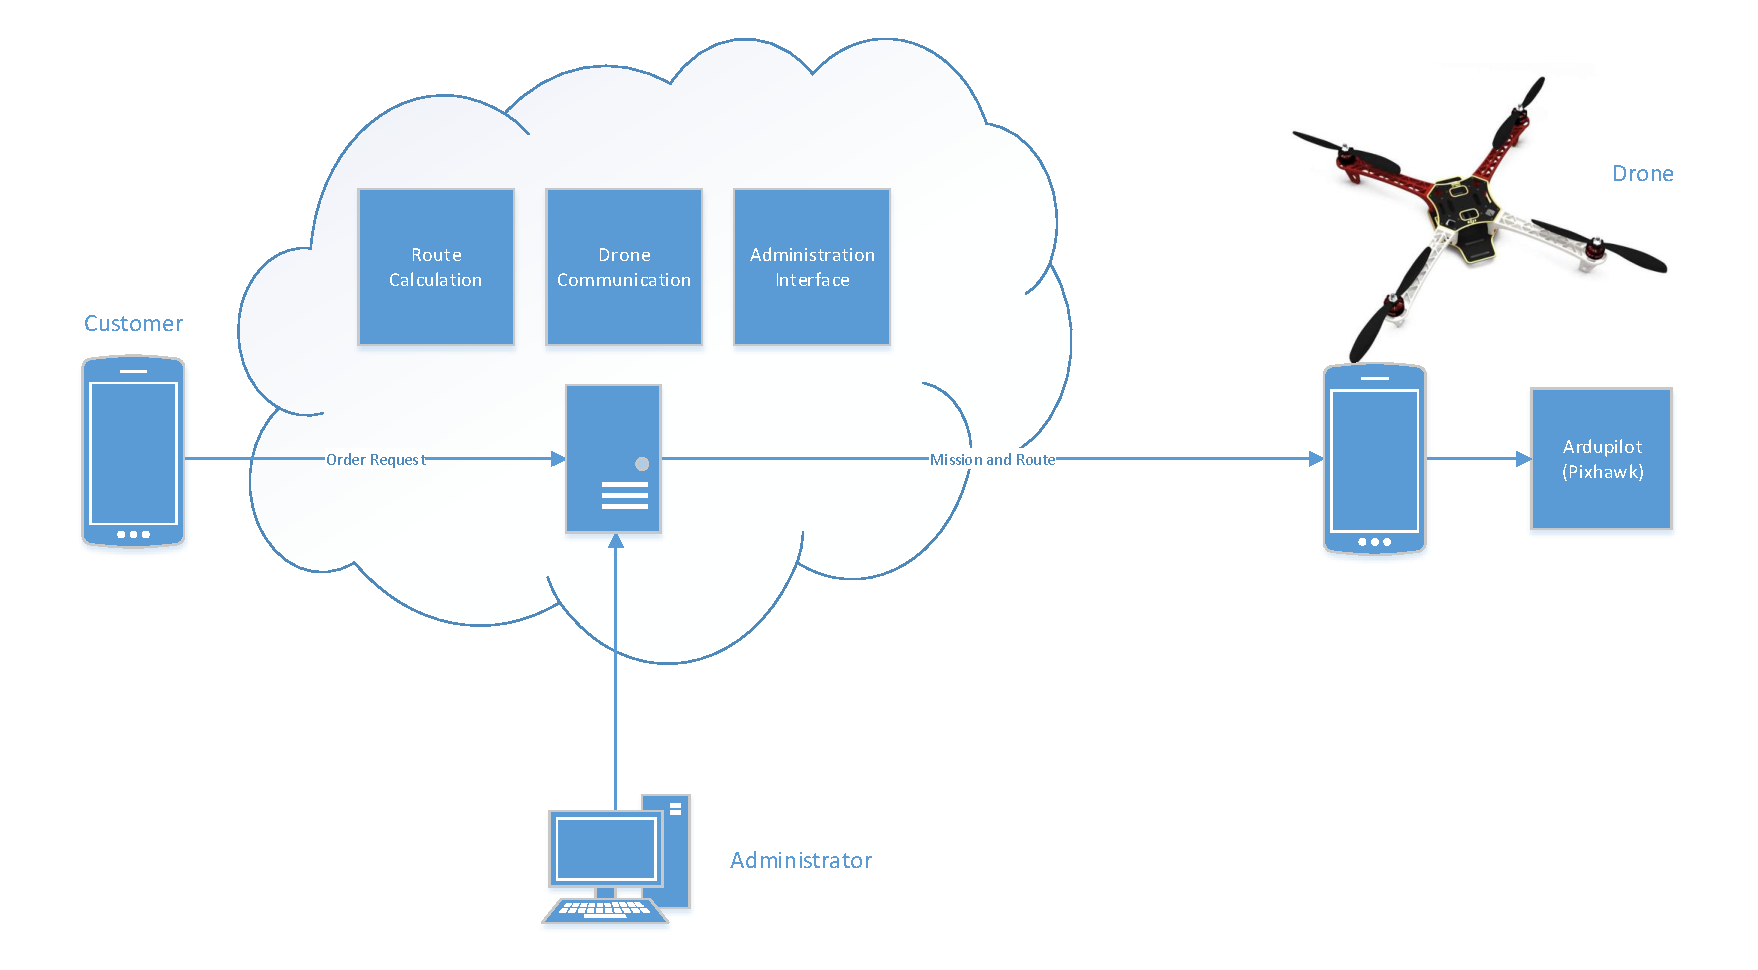
\includegraphics[width=1\textwidth]{images/Overview-Diagram.pdf}
	\caption{Übersicht der Project Helin Architektur }
	\label{fig:architecture-overview}
\end{figure}

\section{Logische Architektur}

\subsection{Komponenten Übersicht}

Abbildung \ref{fig:logical-architecture-overview} zeigt die Hauptkomponenten, sowie eine Übersicht der enthaltenen Layer und Packages. Ausserdem sind die Abhängigkeiten zu den wichtigsten externen Komponenten dargestellt. Hervorzuheben ist ebenfalls die gemeinsame Verwendung der Commons-Komponente. 

\begin{figure}[H]
	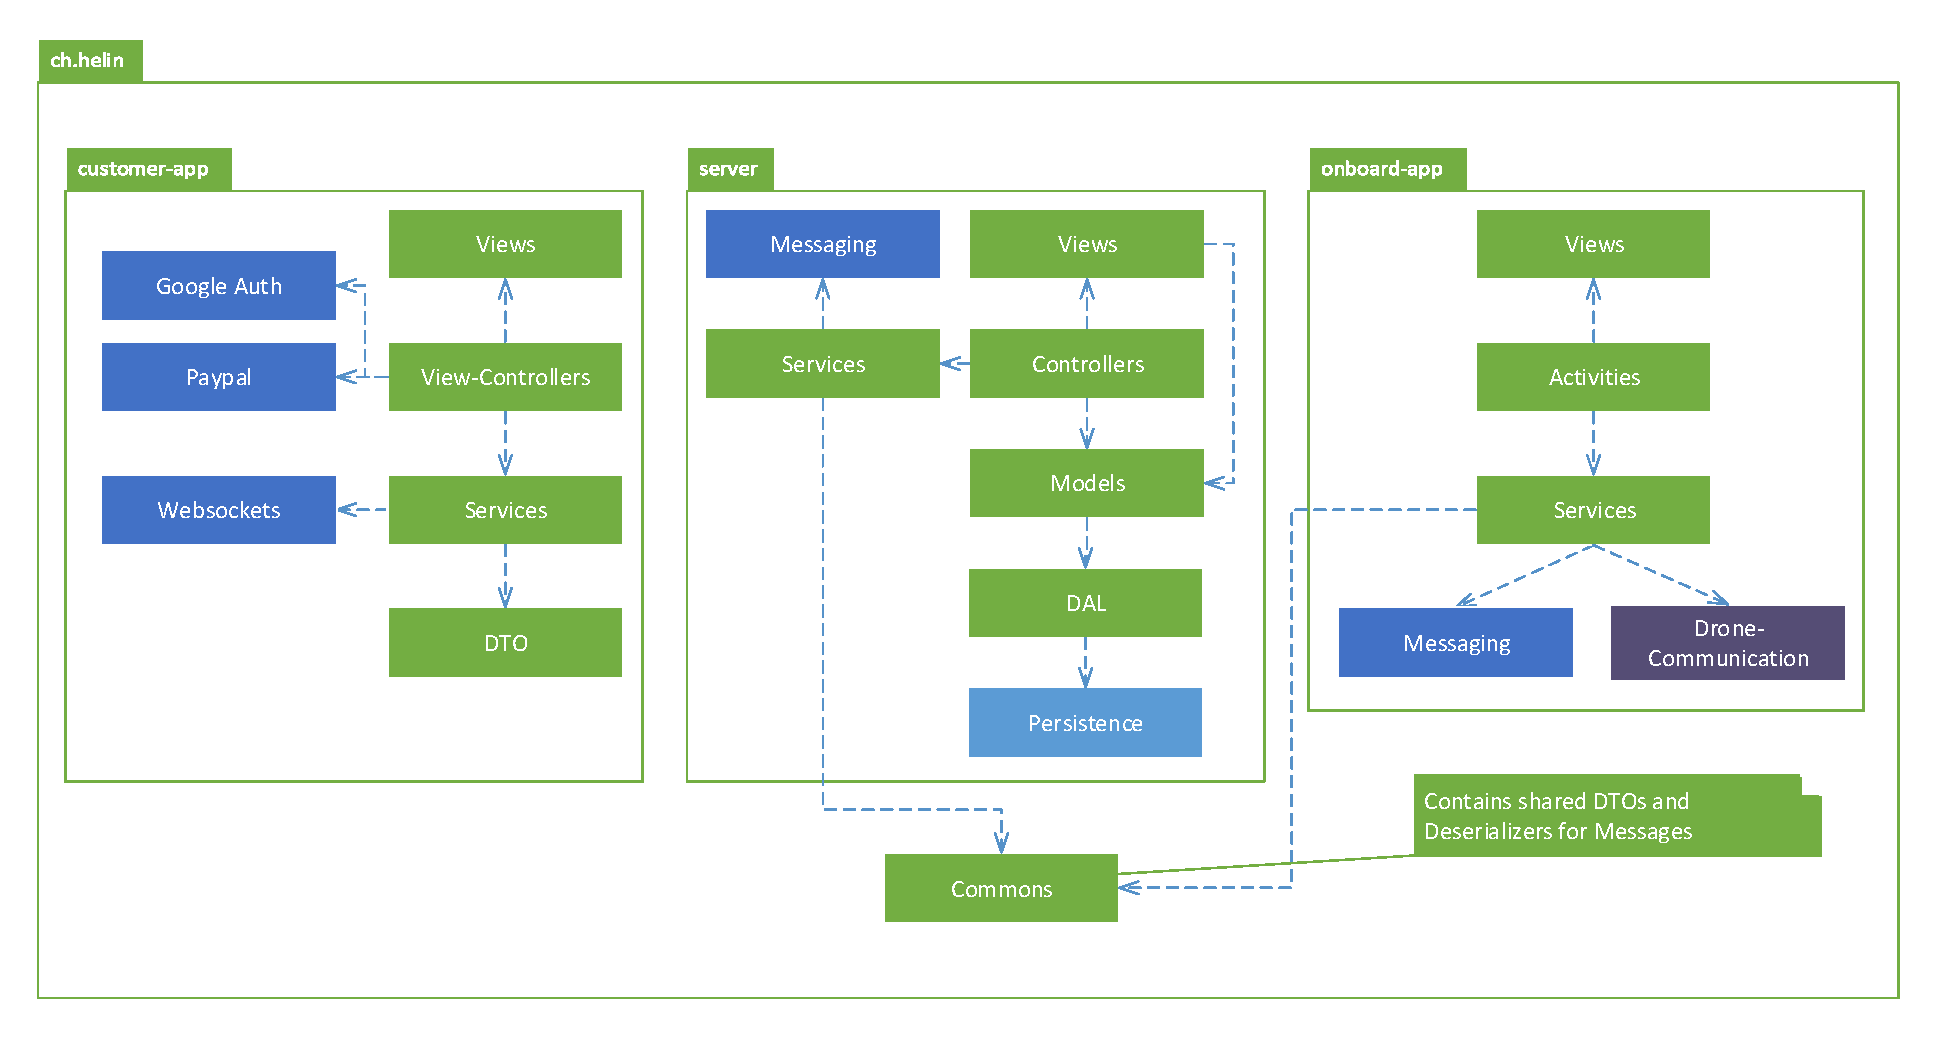
\includegraphics[width=1.0\textwidth]{images/logical-architecture-overview.pdf}
	\caption{Vereinfachte Übersicht der logischen Architektur und deren Komponenten }
	\label{fig:logical-architecture-overview}
\end{figure}

\section{Server-Komponente}

\subsection{Anforderungen}
Aus den in den Anforderungen definierten Zielen, ergeben sich für die Server-Komponente folgende Anforderungen:

\begin{itemize}
	\item Bietet Benutzeroberfläche für Administratoren
	\item Verwaltet \Gls{CRUD} für alle nötigen Klassen (siehe Domain Model Abb. \ref{fig:domain-model})
	\item Verwaltet Verbindungen zu Onboard-Apps und Customer-Apps
	\item Berechnet Flugrouten basierend auf den erhaltenen Bestellungs-Koordinaten
\end{itemize}

\subsection{Layers}
Die Architektur des Servers basiert auf dem {MVC Pattern \cite{MVC}}, da dieses für \Gls{CRUD} Applikationen mit Benutzeroberfläche besonders geeignet ist und dafür viele geeignete Frameworks zur Verfügung stehen.\\

Für Komponenten die aus unterschiedlichen Controllern verwendet werden, wurde zusätzlich eine Service Komponente verwendet. Die Services stellen Abstraktionen für wichtige Funktionen wie das Messaging und die Routenberechnung bereit.\\

Die Verantwortlichkeiten und Kollaborationen der Layer werden nachfolgend genauer definiert.

\subsubsection{View-Layer}
Stellt die grafische Benutzeroberfläche zur Verfügung und rendert diese basierend auf den Model-Daten.

\subsubsection{Controller-Layer}
\begin{tabular}{|p{.70\textwidth}|p{.30\textwidth}|} \hline
	\textbf{Verantwortlichkeiten} & \textbf{Zusammenarbeit} \\ \hline \hline
	\begin{itemize}
		\item Lädt Daten für Views aus dem Data-Access-Layer
		\item Verarbeitet eingehende HTTP-Requests
		\item Verarbeitet eingehende Messages aus den Messaging-Queues
		\item Enthält Business-Logik und steuert Ablauf nach einem Request	
	\end{itemize}&
	\begin{itemize}
		\item Data-Access-Layer
		\item Service-Layer
		\item Model-Layer
		\item Commons
	\end{itemize}
	\\ \hline
\end{tabular}

\subsubsection{Model-Layer}

Der Model-Layer enthält die Datenmodelle. (siehe Domain Model Abb. \ref{fig:domain-model})

\subsubsection{Service-Komponente}

\begin{tabular}{|p{.70\textwidth}|p{.30\textwidth}|} \hline
	\textbf{Verantwortlichkeiten} & \textbf{Zusammenarbeit} \\ \hline \hline
	
	\begin{itemize}
		\item Verwaltet Verbindungen zu den Drohnen
		\item Deserialisiert eingehende Nachrichten
		\item Leitet eingehende Nachrichten von Drohnen an den Controller-Layer weiter	
		\item Leitet eingehende Nachrichten von Customers an den Controller-Layer weiter	
		\item Berechnet Flugrouten basierend auf den vorgegebenen Flugzonen
	\end{itemize}&
	\begin{itemize}
		\item Controller-Layer
		\item Messaging
		\item Commons
	\end{itemize}
	\\ \hline
\end{tabular}

\subsubsection{Data-Access-Layer (DAL)}

Der Data Access Layer bietet die Möglichkeit auf die Persistence Library zuzugreifen und stellt dafür die wichtigsten Funktionen zur Verfügung. 

\section{Onboard-App}

\subsection{Anforderungen}

\begin{itemize}
	\item Kommuniziert mit dem \Gls{Flight-Controller} der Drohne
	\item Kommuniziert mit dem Server
	\item Bietet eine Benutzeroberfläche für den Drone-Operator 
\end{itemize}

\subsection{Layer}

Die App enthält die normalen Android-Application-Layer wie Activities und Views. Zusätzlich kommt der Service-Layer hinzu. Dieser enthält keine Android-Services, sondern selbst entwickelte Service-Klassen. Android Services werden nur zwingend benötigt, wenn etwas im Hintergrund weiterlaufen soll. Da die Onboard-App aber immer im Vordergrund läuft, konnte die aufwendige Kommunikation mit Android-Services mit Hilfe von {Dependency-Injection \cite{DI} umgangen werden.\\

\subsubsection{Service-Komponente}

\begin{tabular}{|p{.70\textwidth}|p{.30\textwidth}|} \hline
	\textbf{Verantwortlichkeiten} & \textbf{Zusammenarbeit} \\ \hline \hline
	
	\begin{itemize}
		\item Verwaltet Verbindung zur Drohne
		\item Verwaltet Verbindung zum Server
		\item Deserialisiert eingehende Nachrichten.
		\item Leitet eingehende Nachrichten vom Server and den Activities-Layer oder andere Services weiter
		\item Ermöglicht das Senden von Nachrichten an den Server
	\end{itemize}&
	\begin{itemize}
		\item Activities-Layer
		\item Messaging
		\item Commons
	\end{itemize}
	\\ \hline
\end{tabular}


\section{Customer-App}

\subsection{Anforderungen}

\begin{itemize}
	\item Kommuniziert mit dem Server
	\item Bietet eine Benutzeroberfläche für den Customer
	\item Ermöglicht die Bezahlung von Produkten
	\item Ermöglicht das Login über einen externen Identifikationsprovider
\end{itemize}

\subsection{Layer}

\subsubsection{View-Layer}
Ist zuständig für die Darstellung der Benutzeroberfläche und bindet die Schnittstellen zum Zahlungsanbieter (Payment) und Identifikationsprovider (Authentication) an.

\subsubsection{Service-Layer}
\begin{tabular}{|p{.70\textwidth}|p{.30\textwidth}|} \hline
	\textbf{Verantwortlichkeiten} & \textbf{Zusammenarbeit} \\ \hline \hline
	
	\begin{itemize}
		\item Verwaltet Verbindung zum Server
		\item Deserialisiert eingehende Nachrichten.
		\item Leitet eingehende Nachrichten vom Server and den Activities-Layer weiter
		\item Ermöglicht das Senden von Nachrichten an den Server
	\end{itemize}&
	\begin{itemize}
		\item View-Layer
		\item WebSockets-Library
		\item Identifikationsprovider
		\item Zahlungsanbieter
	\end{itemize}
	\\ \hline
\end{tabular}



\section{Kommunikations-Architektur}
\label{sec:communication-architecture}

Die Abbildung \ref{fig:communication-architecture-overview} zeigt die Kommunikations-Architektur in der Übersicht.
Wichtig sind vor allem die verschiedenen verwendeten Protokolle, die benötigt werden um die Anforderungen erfüllen zu können. \\

\begin{figure}[H]
	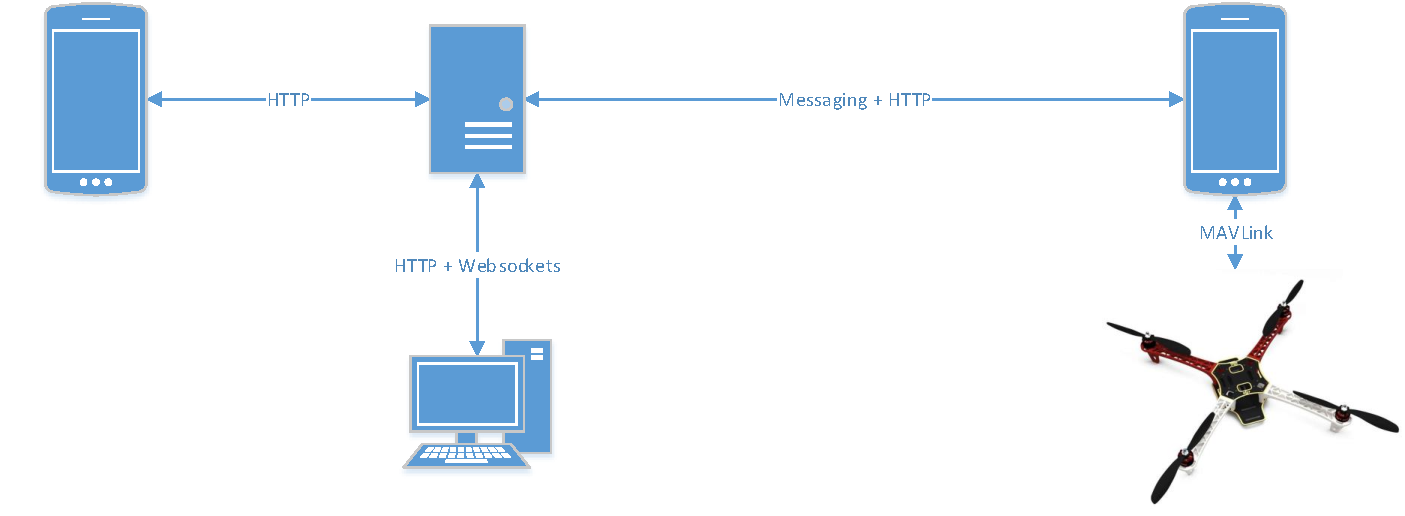
\includegraphics[width=1.0\textwidth]{images/Communication-Overview-Diagram.pdf}
	\caption{Übersicht der Kommunikations-Architektur mit den jeweiligen Protokollen. }
	\label{fig:communication-architecture-overview}
\end{figure}


Für die Kommunikation mit dem Onboard-App wird Messaging verwendet, um bidirektionale Kommunikation zu ermöglichen und die höchstmögliche Zuverlässigkeit zu erreichen.
Eine bidirektionale bzw. beidseitig initiierbare Kommunikation ist bei allen Geräten nötig um Live-Updates zu ermöglichen (Verfolgung der Drohne).
Ausserdem muss die eingesetzte Technologie für die Kommunikation zwischen dem Server und den Onboard-App den Nicht-Funktionalen-Anforderungen gerecht werden, die im Bezug auf Verbindungsabbrüche und Verbindungswiederherstellung bestehen.\\

Aufgrund der schlechten Erfahrung mit WebSocket auf mobilen Geräten und der Probleme mit bei Verbindungsabbrüche, kam diese nicht in Frage. Als Alternative blieb nur Messaging übrig, welches wegen der zeitlichen Unabhängigkeit der Verbindung, vom Server und dem Onboard-App, keine Konsequenzen hat. \\

	
Bei der Anbindung der Customer-App ist die Plattformunabhängigkeit der Schnittstelle höher gewichtet als die Zuverlässigkeit der bidirektionalen Verbindung. Einzig die Liveupdates der Drohnenposition werden über diese Verbindung gesendet. Deswegen wird dort vor allem HTTP verwendet und nur wo nötig WebSockets eingesetzt. Damit können in Zukunft auch andere Geräte verwendet werden um das System anzusprechen, ohne dass sie ein Messaging-Protokoll unterstützen müssen.\\

Die Anbindung an die Administrationsoberfläche erfolgt ebenfalls über HTTP und WebSockets, da dort die Wahrscheinlichkeit eines Verbindungsabbruchs viel geringer ist als bei einem mobilen Gerät. Zusätzlich ist eine Verbindungswiederherstellung der Verbindung viel einfacher, da das Navigieren oder Neuladen der Seite ausreicht. \\


\subsection{Verwendete Enterprise Integration Patterns}
Messaging-Systeme und Protokolle bieten eine grosse Auswahl an Patterns die je nach Anforderungen verwendet werden können. {\cite{EIP} Für dieses Projekt benötigen wir nur einen kleinen Teil davon um den gestellten Anforderungen gerecht zu werden.
%
\subsubsection{Point-to-Point Channel}
Um zwischen einer registrierten Drohne und dem Server einen sicheren und zuverlässigen Nachrichtenaustausch zu ermöglichen, wird jede Drohne bzw. jede App über einen separaten Point-to-Point Channel	\cite[S. 103]{EIP}} angebunden. Der Channel wird nach der Registrierung zugeteilt und stellt den Point-to-Point Kanal zwischen Drohne und Server dar. Dies garantiert dem Server, eine Nachricht an nur eine Drohne zu schicken.
%
\subsubsection{At-most-once}

Die Fehlersemantik At-most-once gibt die Sicherheit, dass eine Drohne eine Mission oder einen Befehl nur ein Mal erhält. Ansonsten müsste das System idempotent gebaut werden. Exactly-once delivery ist ausserdem in der Praxis eigentlich unmöglich umzusetzen, weshalb wir uns für diese Alternative entschieden haben. 
%
\subsubsection{Event-driven Consumer}
{Event-driven Consumer \cite[S. 442]{EIP}} Systeme bieten die Möglichkeit Aktionen auf Grund von Nachrichten auszuführen. Beispielsweise:
%
\begin{itemize}
	\item Drohne erhält neue Mission vom Server und soll dies dem Drone-Operator anzeigen.
	\item Server erhält neue Position von der Drohne und soll diese Nachricht dem Kunden weiterleiten und dem Administrator auf dem Web-Client anzeigen.
	\item Smartphone des Kunden erhält neue Position der Drohne, auf der Karte wird die Position der Drohne angezeigt.
\end{itemize}

\section{Bestellprozess}

Order Cargo (Abbildung \ref{fig:registerDrone}) beschreibt den Bestellprozess und die damit zusammenhängende Kommunikation. \\

Der Kunde bestellt mittels der App ein Produkt (Customer-App), der Server bestätigt ihm die Bestellung und schlägt einen Abwurfort vor. Sollte der Abwurfort dem Kunden nicht entsprechen, so kann er den Prozess abbrechen und ihn noch einmal auslösen, sobald er sich an einer passenderen Stelle befindet.\\

Der Server analysiert die Eignung der verfügbaren Drohnen und bestimmt im Anschluss eine, welche den Auftrag ausführen kann und zeigt die Mission dem Drone-Operator an. Sollte die Drohne bereit sein, so kann er diesen Auftrag bestätigen. Im Falle einer nötigen Wartungsarbeit kann der Auftrag zu diesem Zeitpunkt auch abgelehnt werden. Sobald der Auftrag angenommen wurde, erhält der Drone-Operator genaue Angaben zur Beladung der Drohne. Anschliessend wird die Ladung bestätigt und der Server kann dem Kunden mitteilen, dass die Drone startklar ist. Während des Fluges erhält der Kunde Benachrichtigungen vom Server mit der aktuellen Position der Drohne. Sobald die Ladung abgeworfen wurde, fliegt die Drohne zur Ladezone zurück und bestätigt dem Server die Ankunft. So kann gewährleistet werden, dass bekannt ist, ab wann die Drohne wieder verfügbar ist. \\

Der Bezahl- und Anmeldeprozess wird hier aus Übersichtsgründen nicht dargestellt.
\begin{figure}[H]
	\centering
	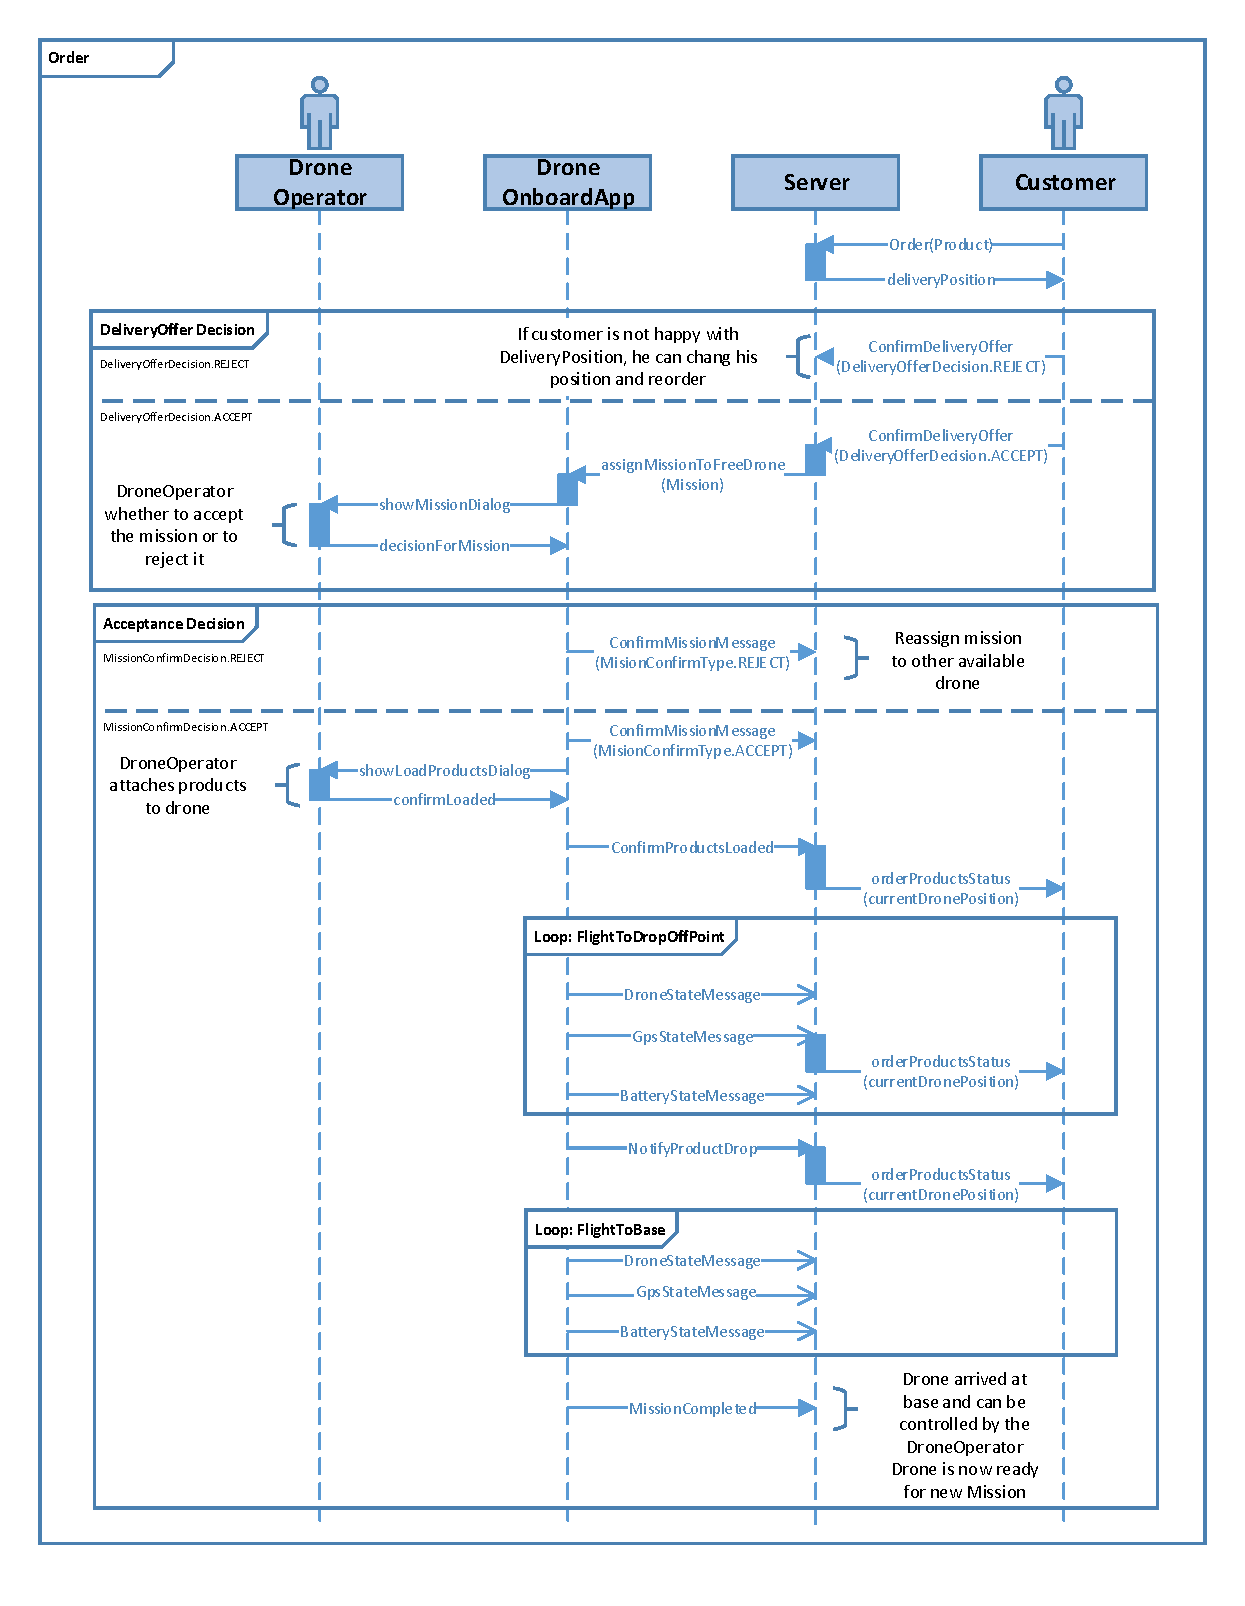
\includegraphics[height=1.0\textheight]{images/sequence_diagram.pdf}
	\caption{Übersicht der Project Helin Architektur }
	\label{fig:registerDrone}
\end{figure}

\section{Missionen}

Wie im Domainmodel (Abb. \ref{fig:domain-model}) ersichtlich, enthalten alle Bestellungen mindestens eine Mission. Die Mission wiederum enthält alle Informationen, die für die Auslieferung notwendig sind. Das folgende Diagramm (Abb. \ref{fig:mission-state}) zeigt die möglichen Zustände einer Mission, von der Bestellung bis zur Rückkehr nach der Lieferung.

\begin{figure}[h]
	\centering
	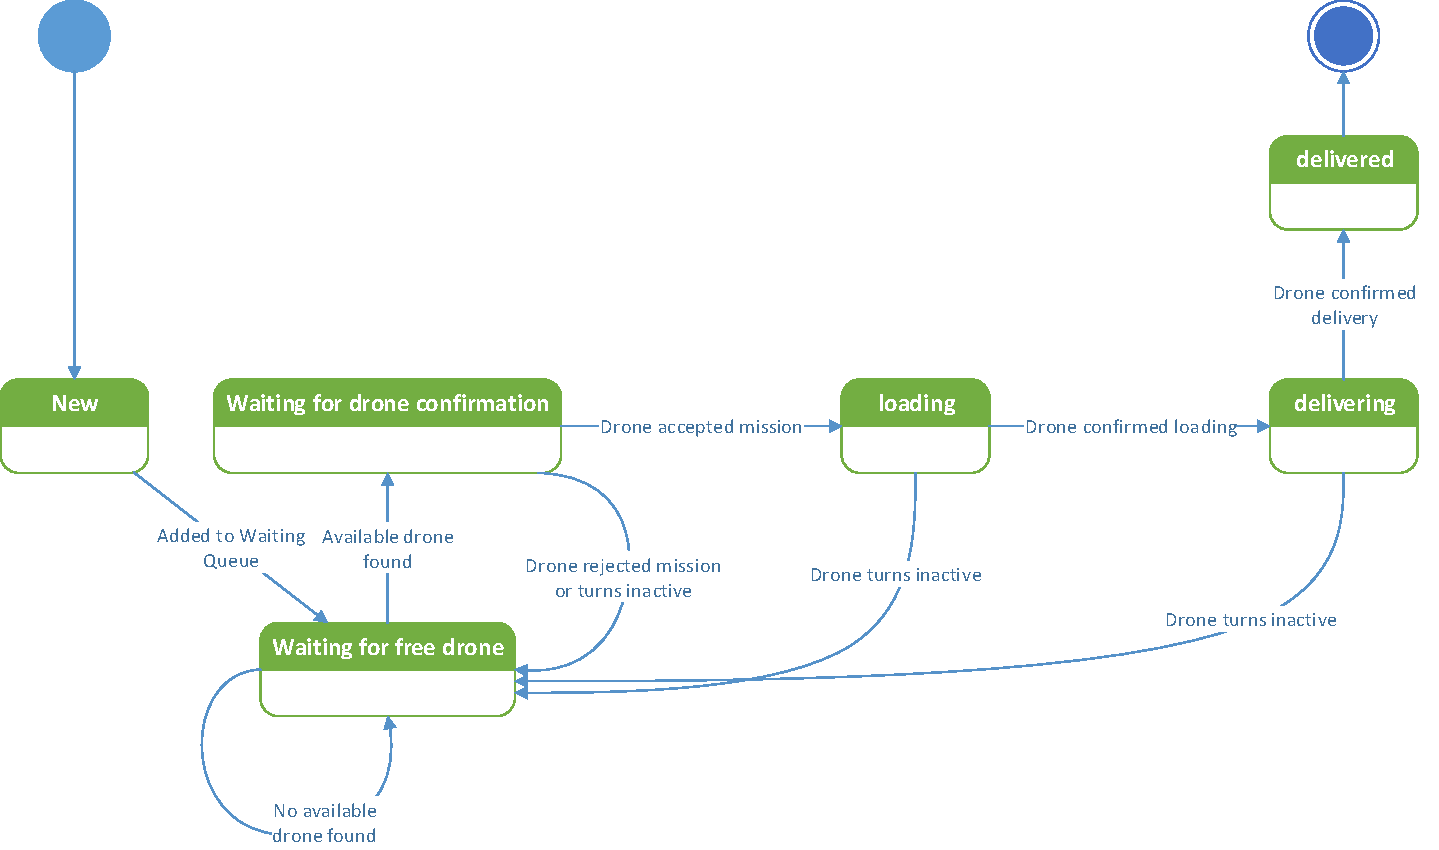
\includegraphics[width=1.0\textwidth]{images/mission-state-flow-diagram.pdf}
	\caption{Zustände der Mission}
	\label{fig:mission-state}
\end{figure}